\documentclass{article}
% We will use NIPS submission format
\usepackage{nips13submit_e,times}
% for hyperlinks
\usepackage{hyperref}
\usepackage{url}
% For figures
\usepackage{graphicx}
\usepackage{subfigure}
% math packages
\usepackage{amsmath}
\usepackage{amsfonts}
\usepackage{amsopn}
\usepackage{ifthen}
\usepackage{natbib}

\title{Machine Learning Project II by Group KATHMANDU}

\author{
  Jade Copet\\
  EPFL \\
  \texttt{jade.copet@epfl.com} \\
  \And
  Merlin Nimier David\\
  EPFL \\
  \texttt{merlin.nimier-david@epfl.com} \\
  \And
  Krishna Raj Sapkota\\
  EPFL \\
  \texttt{krishna.sapkota@epfl.com} \\
}

\nipsfinalcopy

\begin{document}
\maketitle



\begin{abstract}
 In this report, we summarize our findings for the second ML project. We worked on two problems, one about song recommendation and one about detection of people on images. On the detection problem, we had to work with a skewed dataset on which we applied different classifiers such as Logistic Regression, Gaussian Processes, Random Forest, Neural Networks and SVM. We compared their performance using the Receiver Operating Characteristics (ROC) measure. 
\end{abstract}

\section{Song recommendation}

  \subsection{Dataset description}
  \textbf{Objective}: The song recommendation dataset represents the musical habits of users on a musical streaming service. We are given a large number of (user, artist, listening count) triplets, as well as a friendship graph encoding the connections between users. Our goal is to use this training data to perform:

  \begin{itemize}
    \item \textit{Weak} generalization: for existing users, predict the listening counts for unobserved (user, artist) pairs.
    \item \textit{Strong} generalization: for unknown users, predict the listening counts. We may use the friendship data.
  \end{itemize}

  \textbf{About the data}: The listening counts matrix $Y$ covers $1774$ users and $15085$ artists. It is very sparse, as we observe only $69617$ triplets (density of $0.2\%$). The friendship graph $G$ is given in the form of a symmetric $1774 \times 1774$ adjacency matrix, where $G_{i, j} = G_{j, i} = 1$ if users $i$ and $j$ are connected.\\

  Artists have listening counts ranging from $1$ to $2274039$, the most listened artist being Britney Spears (for some reason). Over all observations, before any outlier removal, the average count is 707 while the median count is 278.\\

  TODO: explain carefully how we handled unobserved data.

  \textbf{Error measure}: Both weak and strong prediction involve generating, for a given set of (user, artist) pairs, predicted listening counts. We use mean \textbf{RMSE} as our main error measure. Given a predicted triplets $\hat{Y}$, we compute the RMSE of the residuals on nonzero elements of the target sparse matrix $Y$.\\

  \subsection{Dataset analysis and preprocessing}
  Examining the dataset, we noticed that user $385$ had listened to artist $9162$ a whopping $352698$ times. Assuming an average song duration of $3$ minutes, user $385$ have supposedly spent the equivalent of two full years listening to \textit{Depeche Mode}. It was then necessary to remove such outliers before carrying out any learning.

  Several Machine Learning techniques rely on the assumption that data follows a Gaussian distribution. Applying a $\log$ transform to listening counts brought all counts back to a common scale.

  \begin{figure}[ht]
    \center
    \subfigure{
      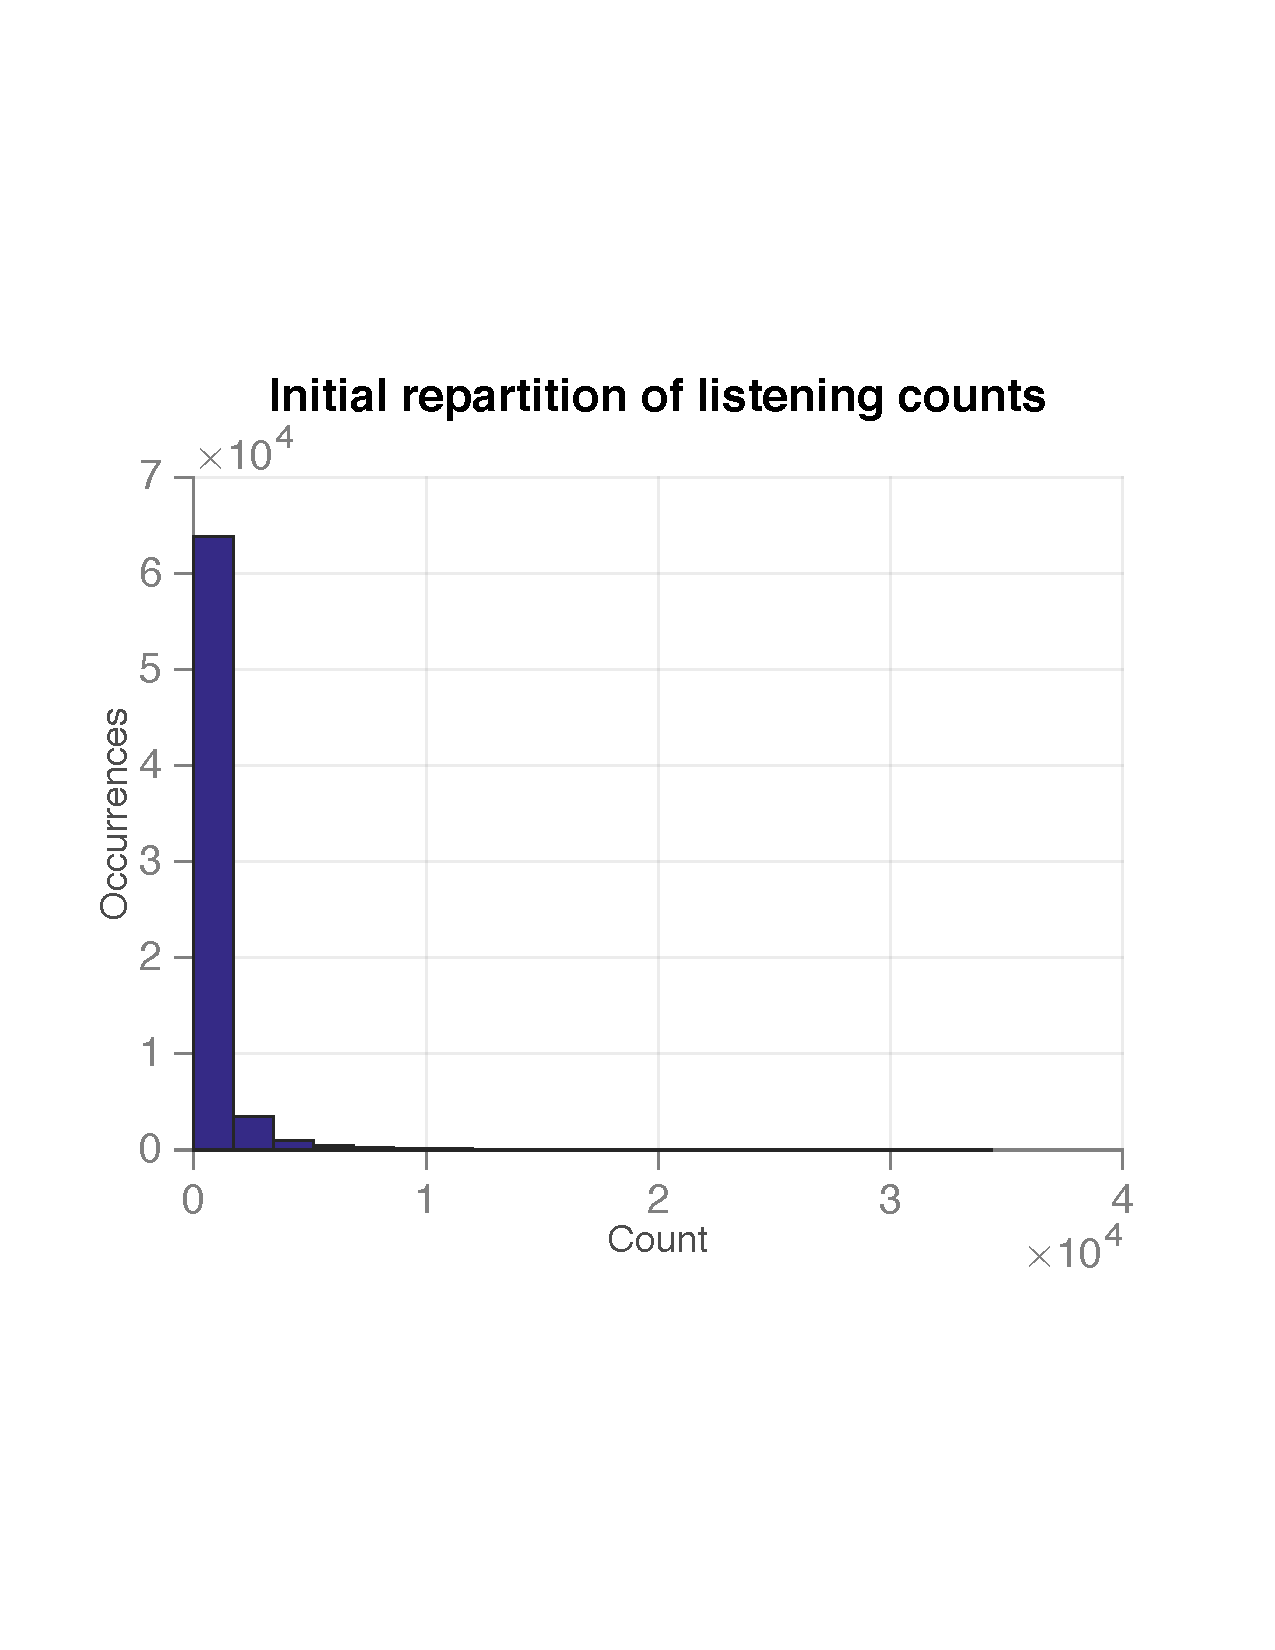
\includegraphics[width=2.5in]{figures/recommendation/unnormalized-counts.pdf}
    }
    \subfigure{
      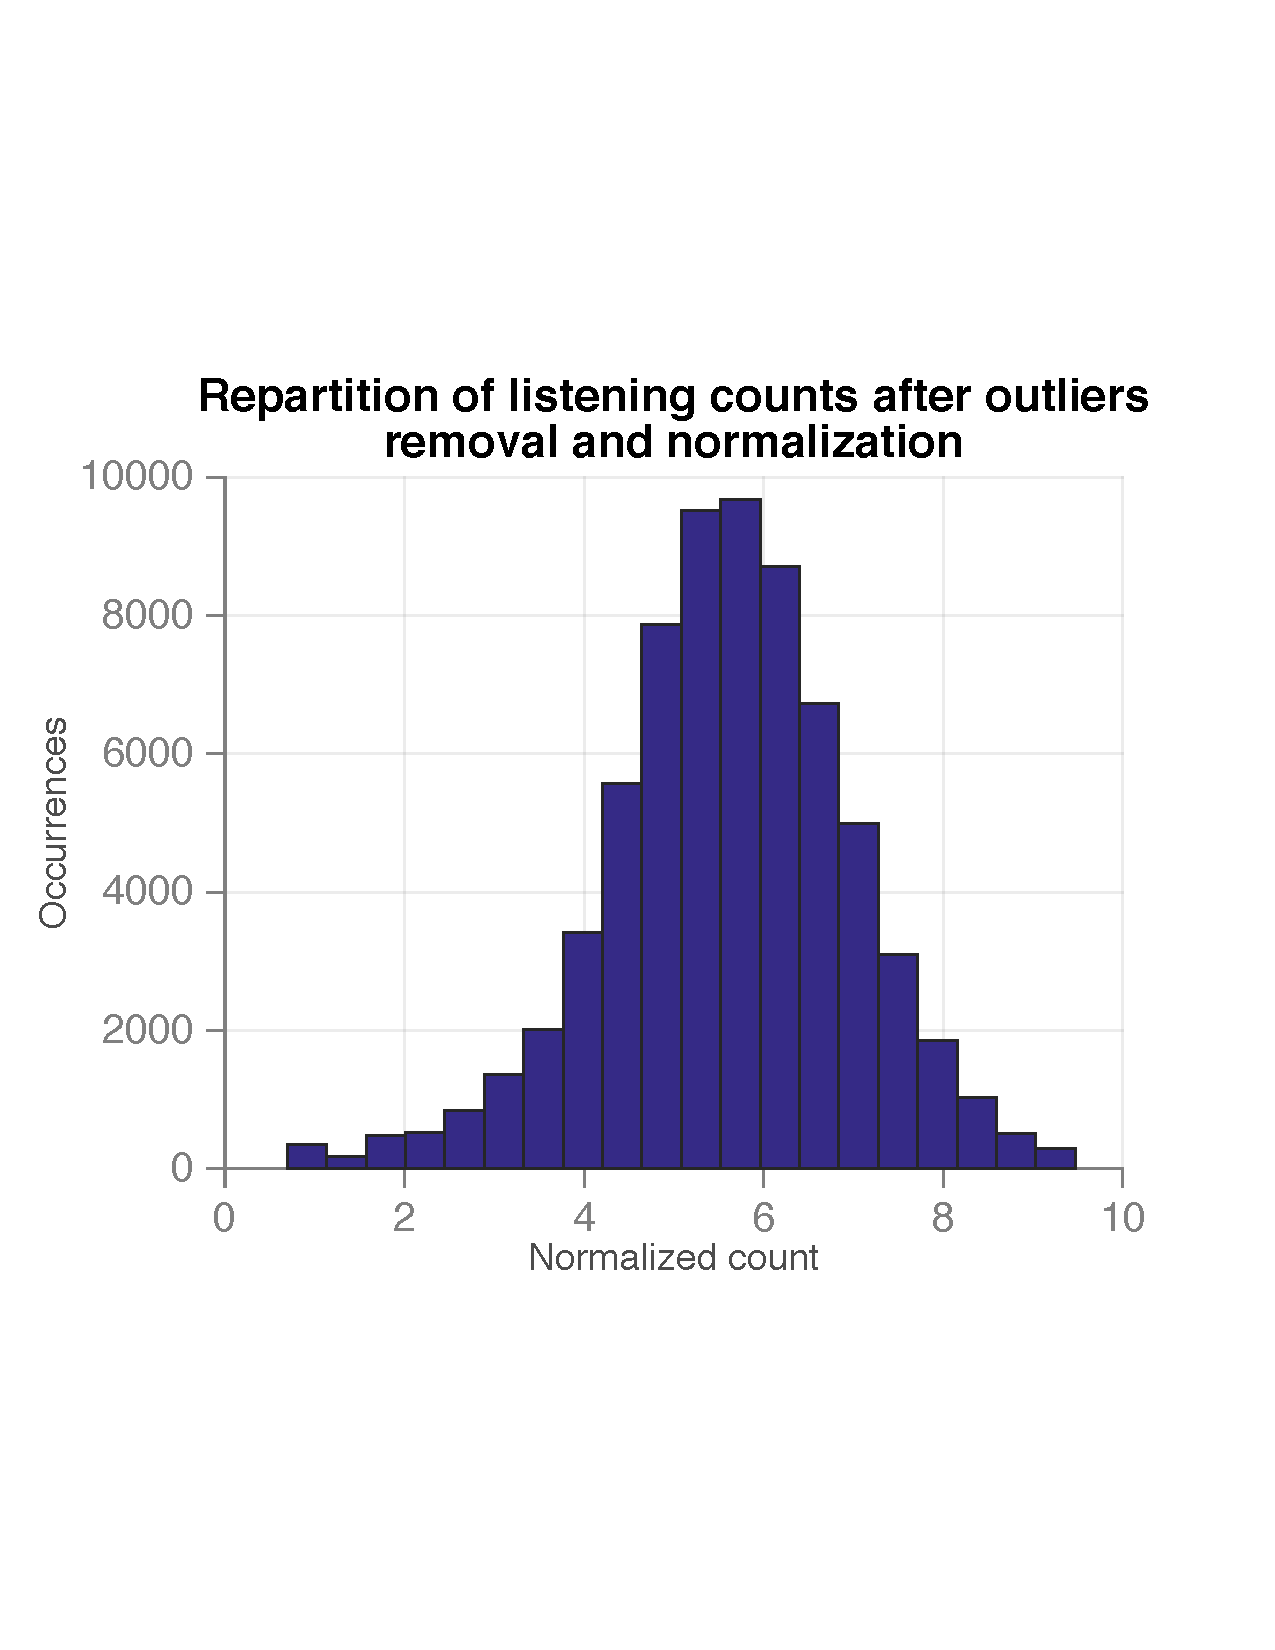
\includegraphics[width=2.5in]{figures/recommendation/normalized-counts.pdf}
    }
    \caption{Normalization makes listening counts distribution more Gaussian}
    \label{fig:recommendation-normalization}
  \end{figure}

  Finally, in order to test our models for both weak and strong predictions, we separated the training set in two ways:
  \begin{itemize}
    \item Entirely remove a proportion of users to use them as a strong prediction test set
    \item Withhold a proportion of the remaining (user, artist, listening count) triplets to use them as a weak prediction test set
  \end{itemize}

  \subsection{Feature transformations}

  \subsection{Final model and predictions}



\section{Image classification}

  \subsection{Dataset description}
  \textbf{Objective}: The people detection dataset consists of a set of images associated with a label that indicates whether there is a person or not in the image. Our goal is to predict whether people are present in unseen images.

  \textbf{Data characteristics}: The training set is composed of $8545$ examples. For each of these images, we are provided with the Histogram of Oriented Gradient (HOG) features generated with Piotr's toolbox \cite{piotrtoolbox}. In order to work with the HOG features we convert them into a vector. Hence for each image we get a vector of dimensionality $9360$.

  The training dataset includes $1237$ positive examples (images with a person on it) encoded with the label $+1$ and $7308$ negative examples encoded with the label $-1$. The distribution is thus heavily skewed towards negative examples.

  \subsection{Performance Evaluation}
  As our dataset is imbalanced, we are relying on both True Positive (TP) and False Positive (FP) values as indicators of our performance. We are using the Receiver Operating Characteristics (ROC) measure and associated \textbf{ROC curves} \cite{rocanalysis} to compare and evaluate our classifiers' performances. The ideal working point is the top-left corner of the ROC curve, where no misclassification is made.

  \subsection{Dataset pre-processing}
  From data exploratory analysis, we did not spot any obvious outlier. For all features, the examples of the training dataset lie between 2 and 3 standard deviations from the median.

  We tried several feature transformations: $\log$, $\exp$, $\sqrt{.}$ and $.^2$ of the input features. The $\exp$ transformed data associated with a Principal Component Analysis seems to enhance performance so we decided to apply it before reducing the data with PCA and working with these new features, otherwise we keep the original features when working with the full-dimensionality matrix.

  We normalized our features before using them for training.

  \subsection{Principal Component Analysis}
  Our features matrix is of dimensionality $9360$ for $8545$ examples which gives us a "fat'' matrix. As several Machine Learning algorithms' time complexity grows fast with dimensionality, we applied a Principal Component Analysis (PCA) in order to work with lower dimensionality data. To do so, we used Piotr's \texttt{pca} implementation which proved to be faster than Matlab's default implementation. We experimented different rank approximation (keeping $50$, $75$, $100$, $300$, $500$ and $1000$ principal components) and applied a simple logistic regression with 3-fold cross validation to have an heuristic about the performance. From the analysis of the resulting ROC curve averaged over the folds \ref{fig:detection-pca-roc-curve} and the associated boxplots \ref{detection-pca-boxplot}, we decided to keep $100$ principal components for our data projection. We have 60\% of our data explained in our reduced space. 
  
  Using a reduced number of features also helps avoiding overfitting, as we are, to some extend, using only the signal (residing in the principal components).
    
   \begin{figure}[ht]
       \center
      	\subfigure[ROC Curve of logistic regression applied to different low-rank approximation. $100$ principal components returns the best results begin the most top-left curve.]{
      		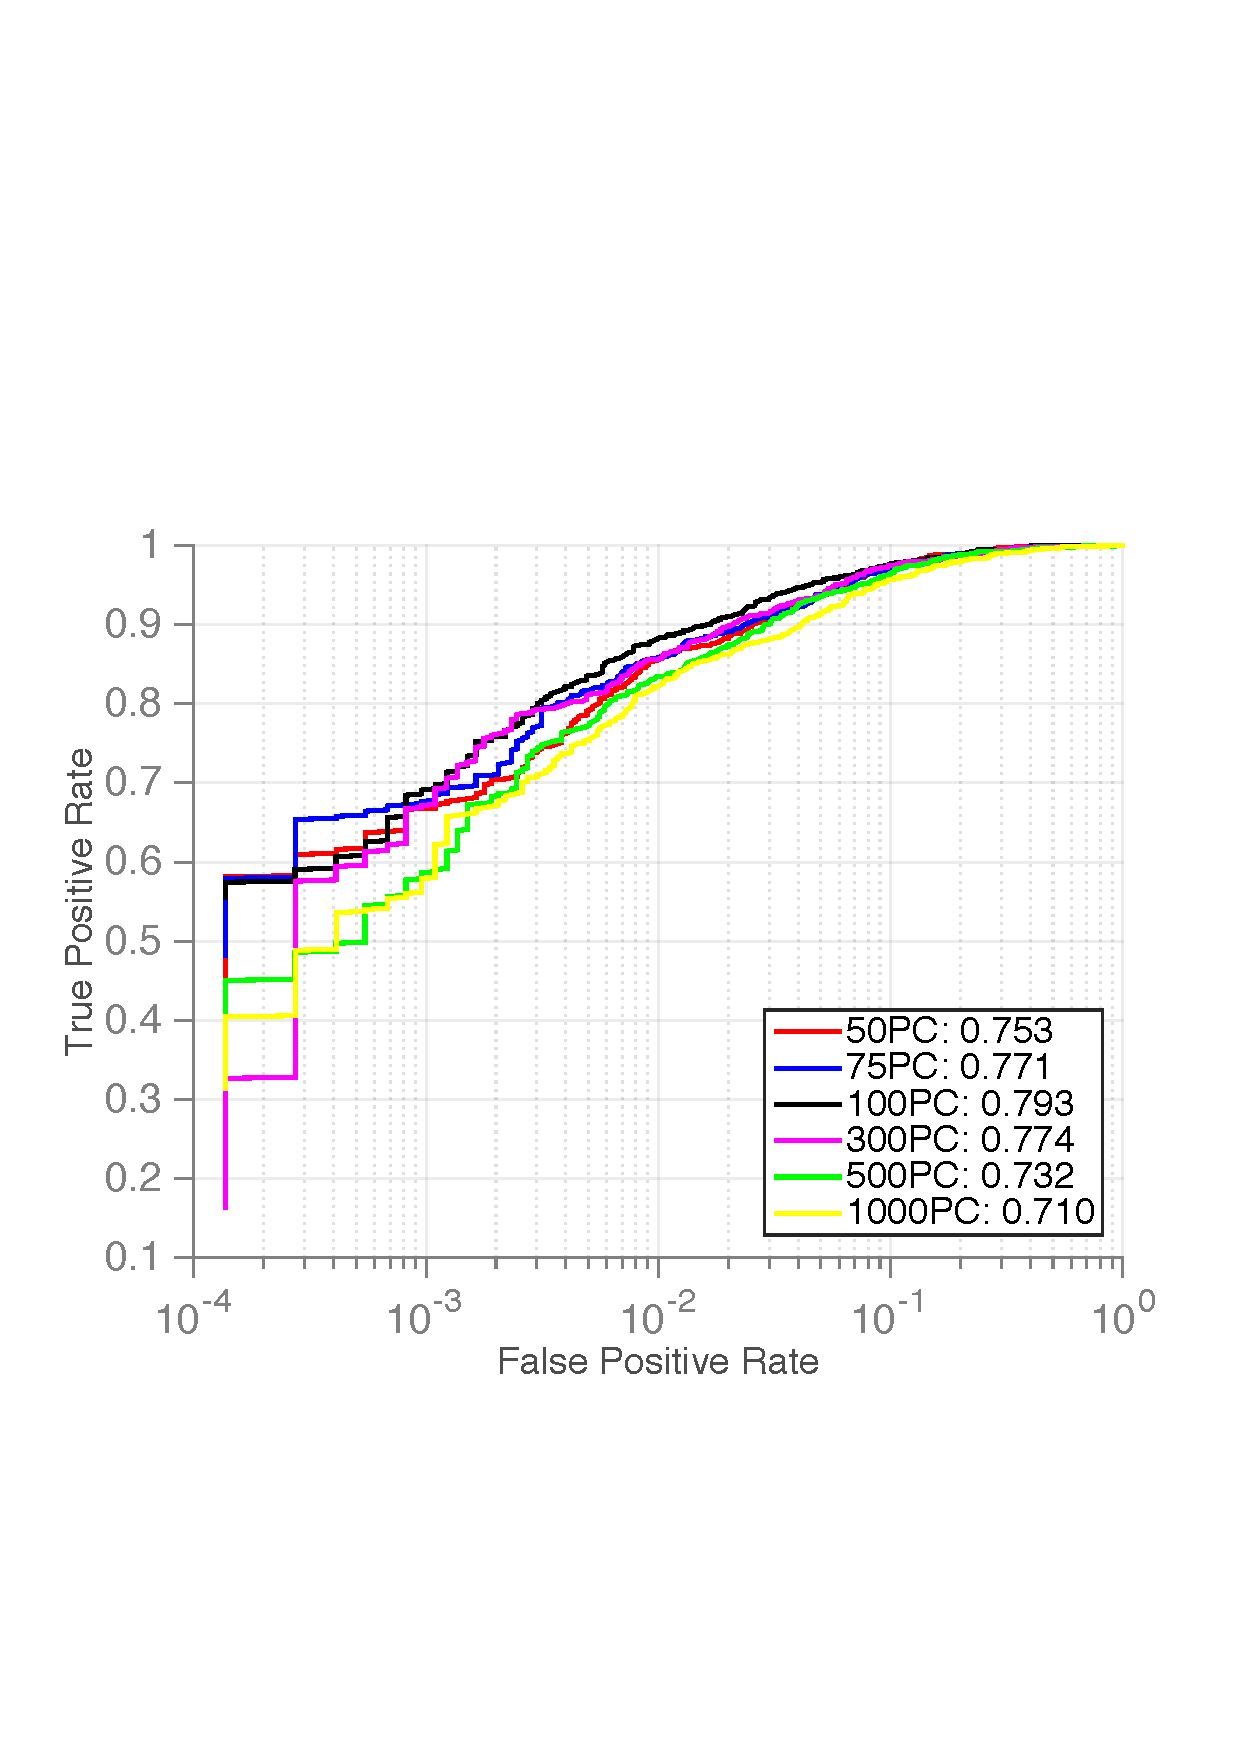
\includegraphics[width=2.5in]{figures/detection/pcaselection-curve2.pdf}
      		\label{fig:detection-pca-roc-curve}
      	}
    	\hfill
	\subfigure[Associated boxplots informing about the variance of each method confirms $100$ principal components as a robust option.]{
      		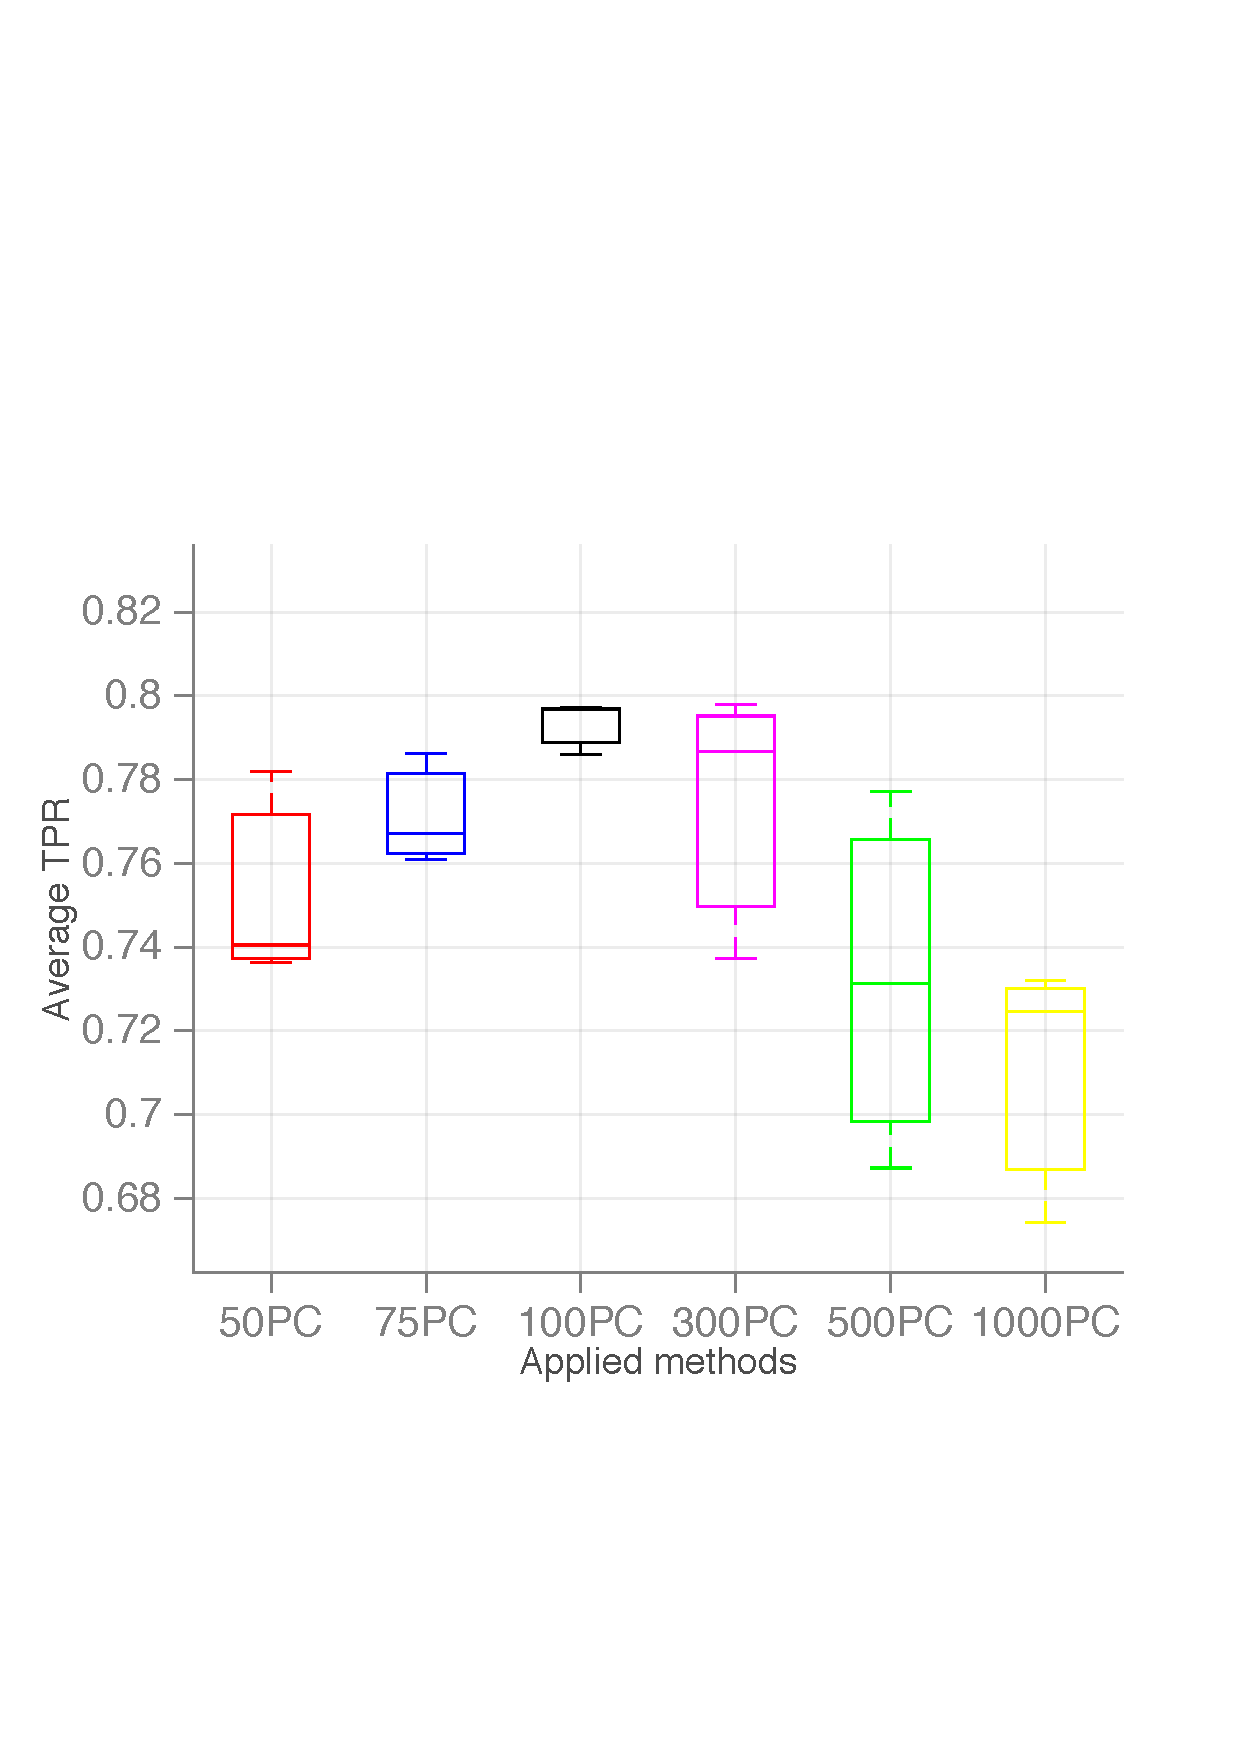
\includegraphics[width=2.5in]{figures/detection/pcaselection-boxplots2.pdf}
      		\label{detection-pca-boxplot}
    	}
	\caption{PCA on detection dataset. Selection of the number of principal components}
  \end{figure}

  \subsection{Training different classifiers}
  We learnt classifiers from several techniques and compared them to find the best performing model. We started with a simple Logistic Regression. Then, we applied Gaussian Processes classification using Rasmussen's GPML library \cite{gpmltoolbox}, Random Forests using Matlab's implementation, Neural Networks thanks to the Deep Learning toolbox \cite{deeplearningtoolbox}, and finally Support Vector Machines using LIBSVM toolbox \cite{libsvmtoolbox}.\\

  \textbf{General approach}:
   	\begin{itemize}
	   	\item Applying a default implementation of the model to normalized input data or reduced input data after applying PCA depending on computation complexity and performance of the algorithm.
    		\item Tuning model parameters: for parameters that seemed relevant, we chose a range of values to test on and find the best combination using cross validation. As training the different models is rather slow, we used 3-fold cross validation. Other parameters were set manually. We plot learning curves and select parameters values that maximize the average True Positive Rate (TPR) on the test set. It is important to point out that we may not select the very best parameter doing so because the average TPR is only a proxy but it is the only measure we can rely on to automate the search.
		  \item Validating the trained model using 3-fold cross-validation: we computed an average ROC curve over train and test data. We represent the curve with its 95\% confidence interval (see our \texttt{kCVfastROC} function).
  		\item Finally, we compare the candidate model with other classifiers plotting a ROC Curve averaged over 3-fold cross validation and a boxplot for each of them (see our \texttt{kCVevaluateMultipleMethods} function).
	\end{itemize}

  \textbf{Logistic Regression}: Since it can be seen as a single-layer Neural Network, we used the Deep Learning toolbox. We added a regularization term (see below for details). We applied this classifier on our reduced data after exponential transform and learned the regularization term with cross validation and ended up with a regularization of value equal to $10^{-3}$.

  \textbf{Gaussian Processes}: Having a large number of data examples in our training set, we used "large scale'' GP classification from Rasmussen's GPML library. It relies on low-rank and diagonal approximation to the exact covariance using induction points. Solving a classification problem, we opted for a logistic function as a likelihood function. We did not have specific intuition about the prior distribution so we used a constant 0-mean prior. We selected a squared exponential covariance with isometric distance measure \texttt{covSEiso} rather than the ARD one. While yielding comparable performance, the former uses only two hyper-parameters, in contrast with the latter which needs $D+1$ hyper parameters and thus might be prone to overfitting. Finally we chose Laplace approximation to infer on our data because of its reasonable computation time (as opposed to Expectation-Propagation). Gaussian Processes have a lot of hyper parameters and are very sensitive to those. We only succeed to make it work on a low-rank approximation over 50 principal components. None of our several trials of grid search to find the hyper parameters for our regular reduced input data succeeded.
  
    \textbf{Random Forests}: We trained a random forest on the reduced input data and learned different parameters through cross-validation. We experimented with the number of trees (on which the decision is averaged), the fraction of variables selected in the random bagging for each decision split, and the minimum observations per tree leaf. A low number of these observations and a large fraction of features selected might be prone to overfitting while increasing the number of trees improves the predictions performances up to some point. However increasing the number of minimum observation per leaf gives us worse results, this may happen because we don't have enough training examples in our folds. We kept 100 as the number of trees over the range $[50, 100, 200, 300, 400, 500]$, as it offers a good compromise between computational complexity and performance:  while performing as good as more trees it is reasonably fast. We chose the $\sqrt{size(X,2)}/ 2$ as the optimal number of variables sampled.

  \textbf{Support Vectors Machines}: We experimented with different kernels: linear, polynomial and Radial Basis Function (RBF). As the polynomial and RBF kernels are more complex models their computational complexity is much higher than the linear one. Hence we applied SVM with those kernels on our low-rank approximation data. We retained the RBF kernel because it was giving the best performance results (fig. \ref{fig:detection-svm-kernels}) and then we select the best smoothness parameter $\gamma$ over a range of possible values through cross validation. We used the range $[0.2*L, 0.5*L, L, 2*L, 5*L]$ with $L = 1 / \sqrt{size(X,2)}$. As $\gamma$ increases, the algorithm tries harder to avoid misclassification on train data which leads to overfitting. One can notice it on fig. \ref{fig:detection-svm-gamma} that represents the learning curve for $\gamma$ parameter: the model fits perfectly the training data and thus performs worse on test data.
  
     \begin{figure}[ht]
       \center
      	\subfigure[Averaged ROC curves to choose the best kernel.]{
      		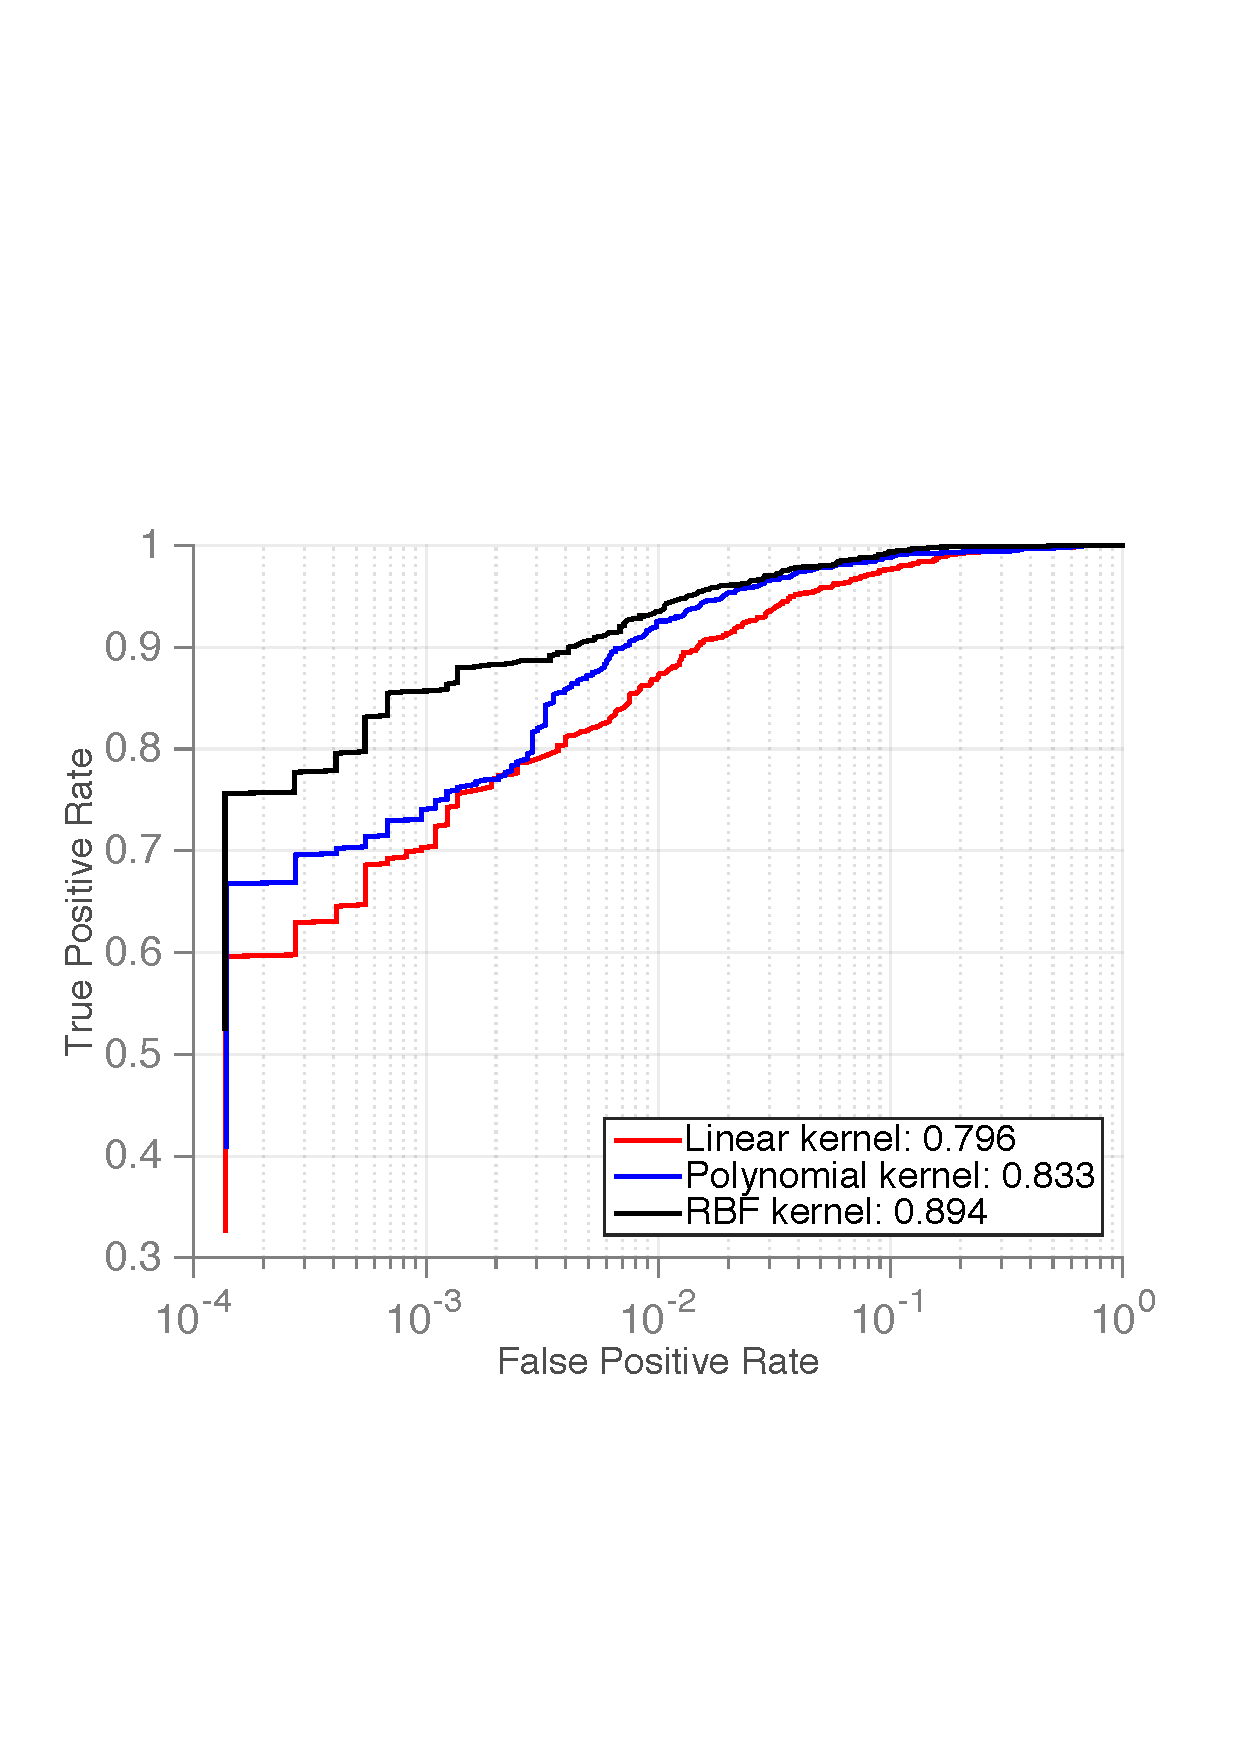
\includegraphics[width=2.5in]{figures/detection/svm-kernels-curve.pdf}
      		\label{fig:detection-svm-kernels}
      	}
    	\hfill
      	\subfigure[Learning curves for  $\gamma$ parameter of RBF kernel.]{
      		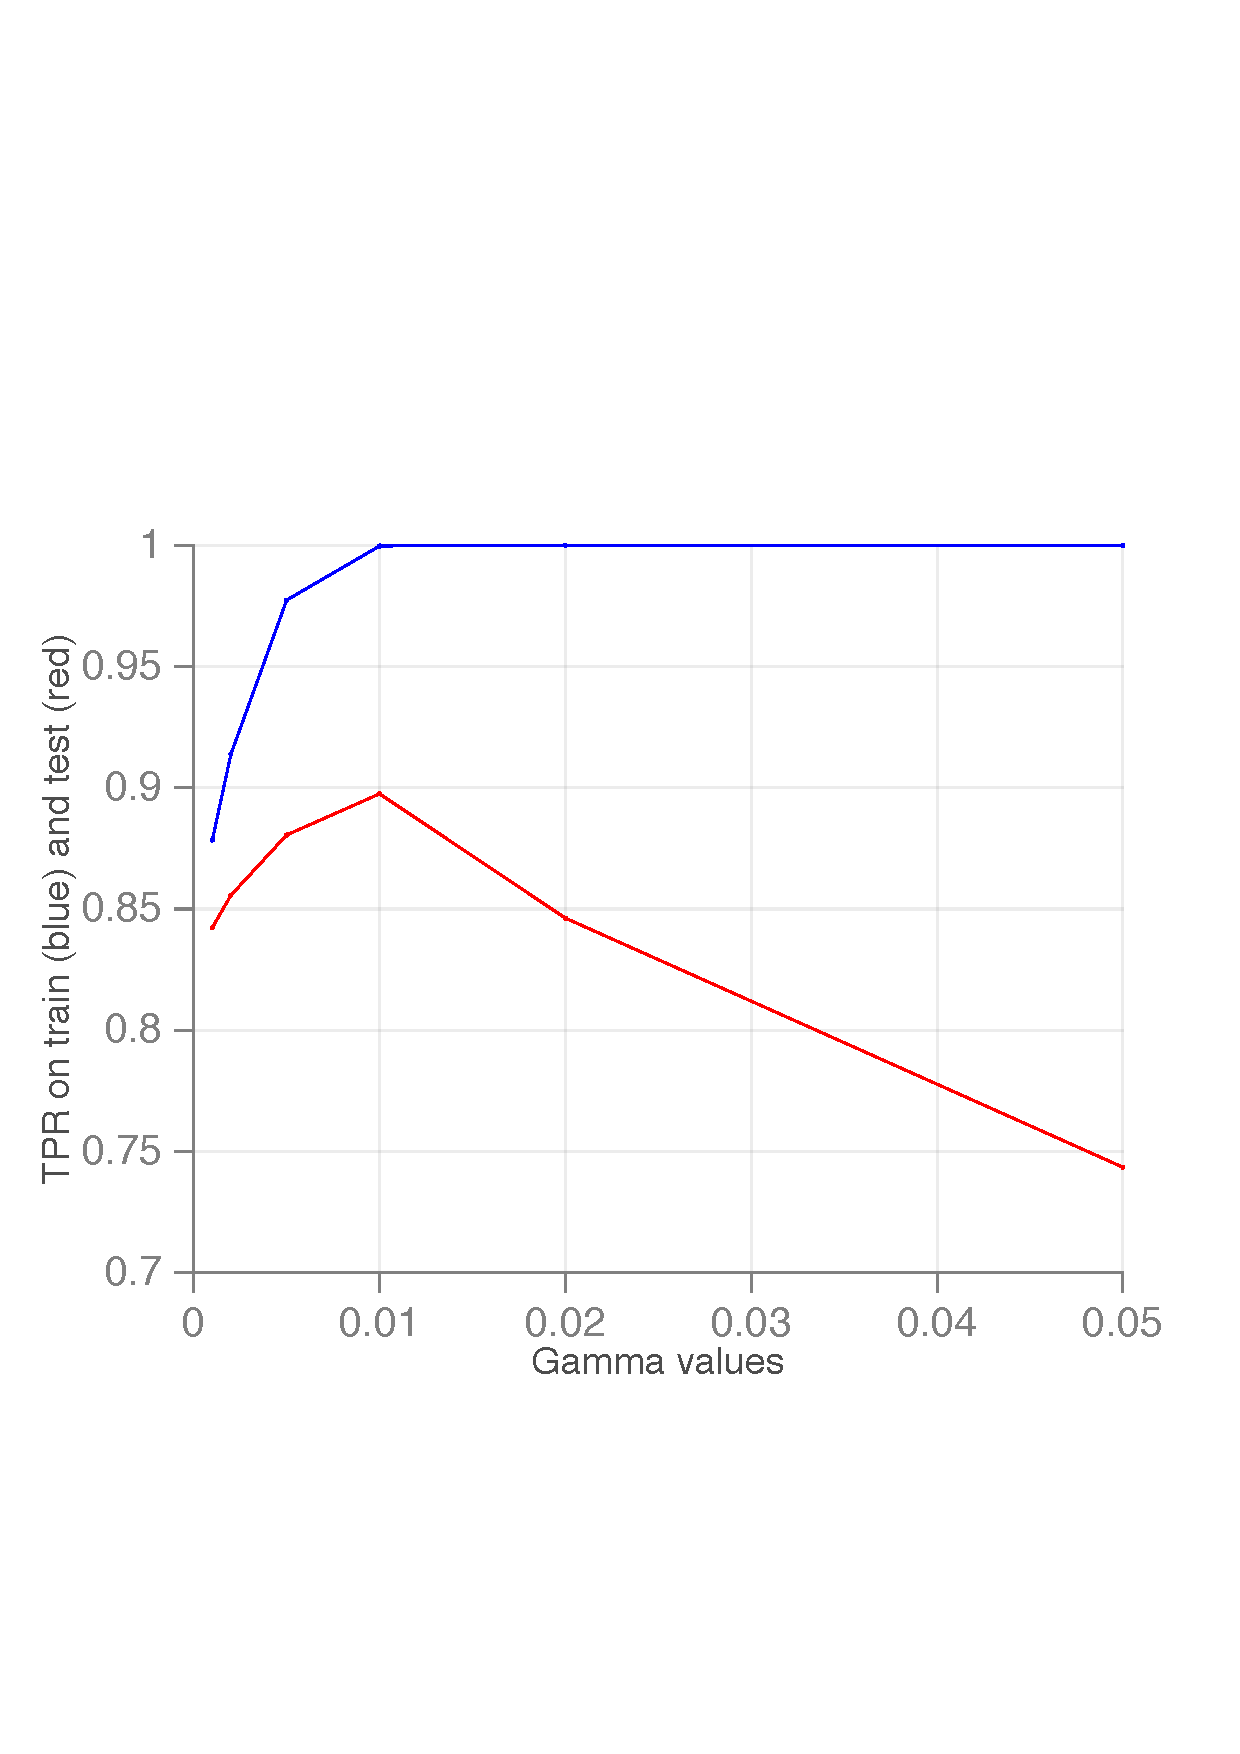
\includegraphics[width=2.5in]{figures/detection/svm-gamma-learningcurve.pdf}
      		\label{fig:detection-svm-gamma}
      	}
	\caption{Selecting the best parameters with ROC comparison and learning parameters for SVM.}
  \end{figure}

  \textbf{Neural Networks}: We applied a 2-layered Neural Network on our full-dimension data. We were able to tune the number of activation functions on each layer as well as its type. A sigmoid activation function gives better results than the $\tanh$ function and is more robust.\\
  To avoid overfitting, we leveraged two regularization methods:
  \begin{itemize}
   	\item Applying weight decay on the second layer (corresponding to Tikhonov regularization)
	  \item Defining a "dropout fraction'', which removes randomly some units during the training \cite{dropout}
  \end{itemize}
	The best combination of weight decay and dropout fraction parameters were selected from ranges of parameters using cross-validation as described in the general approach section. We used  the ranges $[0, 0.1, 0.2, 0.3, 0.4, 0.5]$ for dropout fraction and $[0, 10^{-5}, 10^{-4}, 10^{-3}]$ for weight decay and ended up with selected values of $0$ for the dropout and $10^{-3}$ for the weight decay.\\

  \subsection{Model selection and predictions}
    \textbf{Models comparison}: Finally we compare all our models tuned with the best parameters found using 5-fold cross validation. The results are presented on Figure \ref{fig:detection-compare-roc-curve}. SVM with the RBF kernel gives the best performance with its ROC curve lying above the other classifiers and an average TPR reaching $0.911$. The second best classifier is the Neural Network on full-dimensionality data presenting the lowest variance over all methods. It worths pointing out the good performance of penalized logistic regression which is a very simple model. We did not expect much on the Gaussian Processes as it was really difficult to find parameters to have results so we were not able to tune it a lot. However we are quite surprised about the Random Forest classifier which we would have expected to provide much better results as it is supposed to be particularly well fitted for such problems. We think that we did not succeed to find the best settings for this classifier.

   \begin{figure}[ht]
       \center
      	\subfigure[Averaged ROC Curves of all our tuned classifiers.]{
      		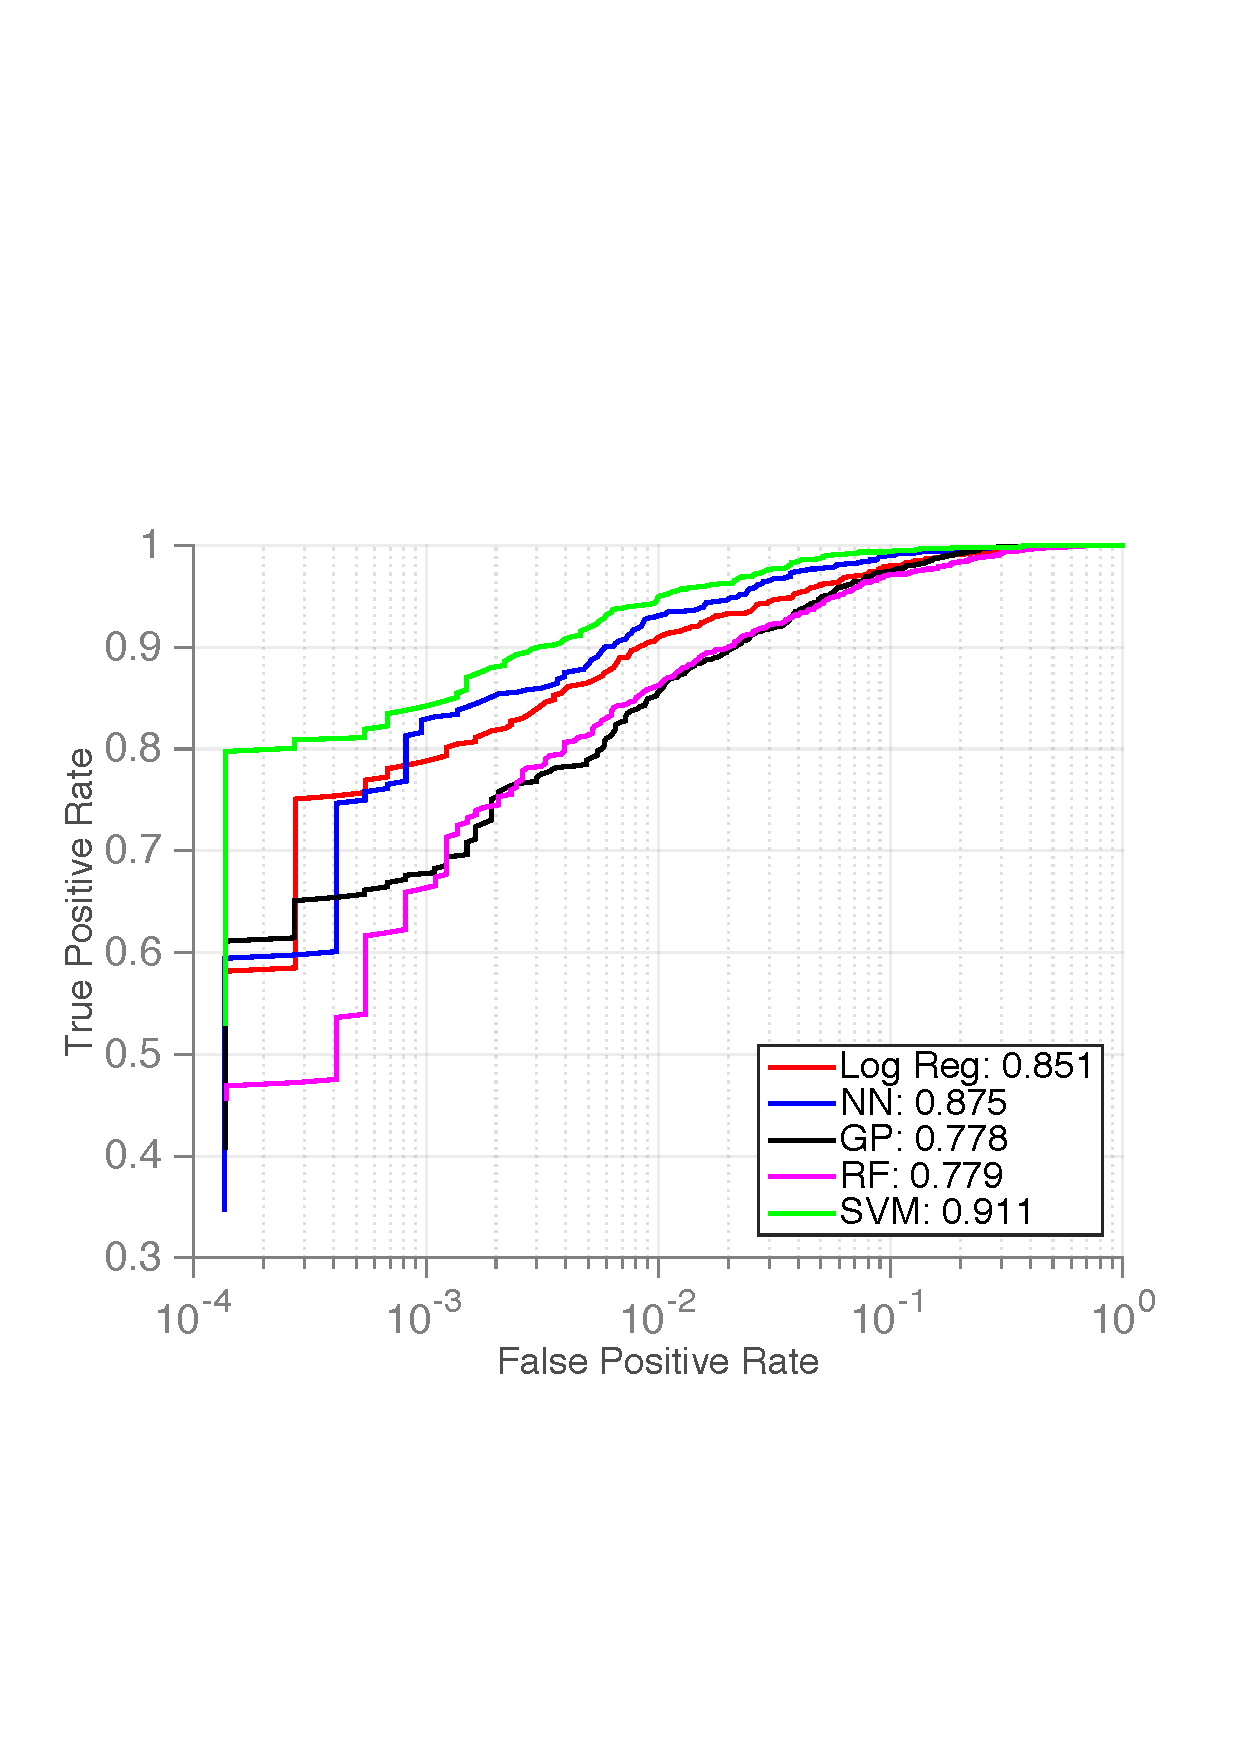
\includegraphics[width=2.5in]{figures/detection/compareall-5fold-curve.pdf}
      		\label{fig:detection-compare-roc-curve}
      	}
    	\hfill
	\subfigure[Boxplots of each classifier.]{
      		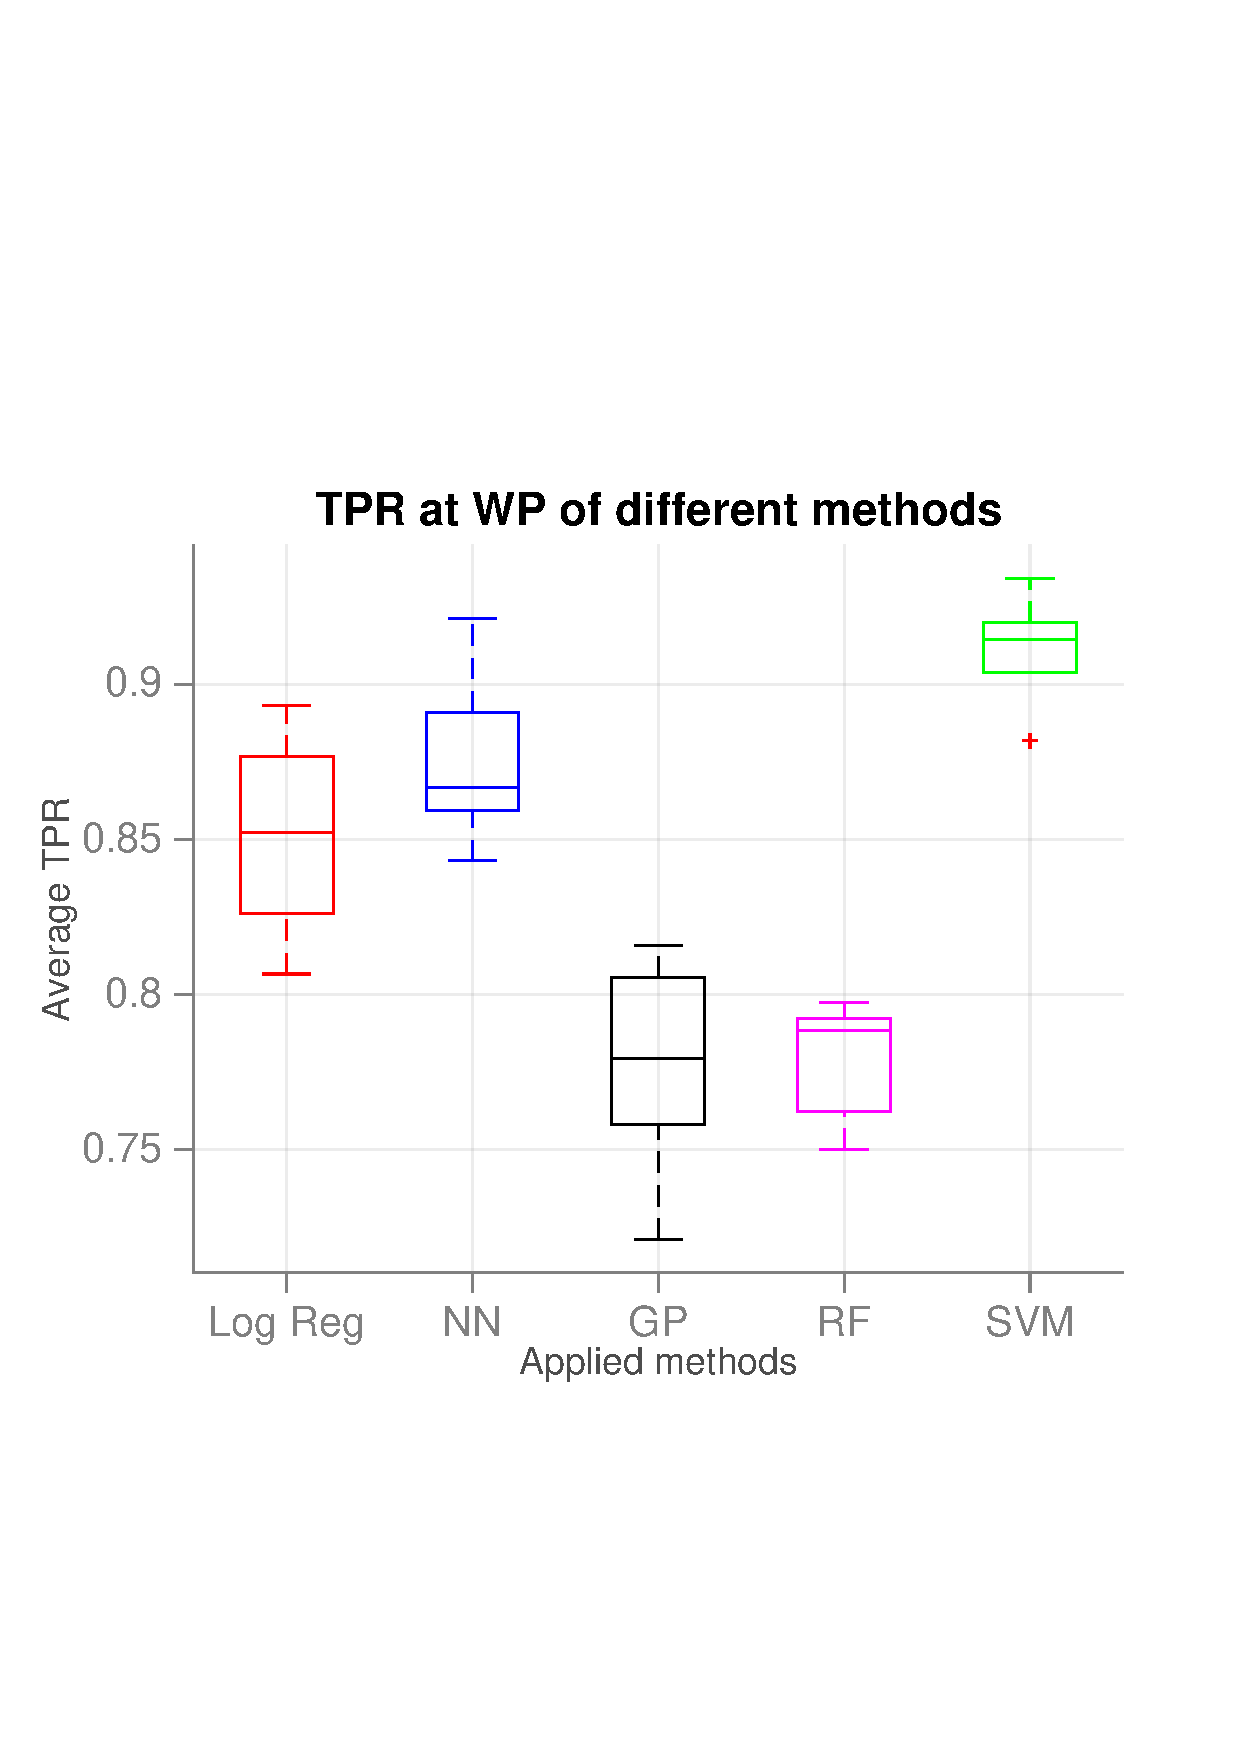
\includegraphics[width=2.5in]{figures/detection/compareall-5fold-boxplots.pdf}
      		\label{detection-compare-boxplot}
    	}
	\caption{Comparison of all models. SVM appear to provide the best performance.}
  \end{figure}
  
  \textbf{Predictions}: Hence, we produced our predictions for the given \texttt{X\_test} input data using the SVM classifier and wrote them in the mat file \texttt{personPred.mat}.

\section{Summary}
  Sparse matrix representation made manipulation less straightforward and required us to learn a few new techniques.
  
  In the detection problem, we first applied a PCA to reduce the dimensionality of our data. Then, we applied different classifiers and experimented with their parameter to improve their performance. Once having the optimal settings we could get, we compared them using ROC curves. Finally we selected SVM with RBF kernel for our predictions.
  
  \subsubsection*{Acknowledgments}
  	We would like to thank Prof. Emtiyaz Khan and the teaching assistants for creating this project. It was a great opportunity for us to put in practice the machine learning techniques seen in class on real-world problems. We also would like to thank them for their availability throughout the semester.\\
  
     \begin{thebibliography}{99}
   
   	\bibitem{piotrtoolbox} Doll'ar P, \textit{Piotr's Computer Vision Matlab Toolbox}
	
	\bibitem{rocanalysis} Fawcett T, \textit{An introduction to ROC analysis}, in Pattern Recognition Letters 27 (2006) 861-874.
	   
     	\bibitem{gpmltoolbox} Rasmussen C and Williams C, \textit{Gaussian Processes for Machine Learning Toolbox}
	
	\bibitem{deeplearningtoolbox} Rasmus Berg Palm, \textit{Deep Learning Toolbox}
		
	\bibitem{libsvmtoolbox} Chang CC and Lin CJ, \textit{LIBSVM: A library for support vector machines}, in ACM Transactions on Intelligent Systems and Technology, vol. 2 (2011)
		
	\bibitem{dropout} Srivastava N, Hinton G, Krizhevsky A, Sutskever I and Salakhutdinov R, \textit{Dropout: A Simple Way to Prevent Neural Networks from Overfitting}, in Journal of Machine Learning Research 15 (2014) 1929-1958.

   \end{thebibliography}
   
\end{document}
